\documentclass{article}

% Language setting
% Replace `english' with e.g. `spanish' to change the document language
\usepackage[spanish]{babel}

% Set page size and margins
% Replace `letterpaper' with `a4paper' for UK/EU standard size
\usepackage[letterpaper,top=2cm,bottom=2cm,left=3cm,right=3cm,marginparwidth=1.75cm]{geometry}

% Useful packages
\usepackage{amsmath}
\usepackage{graphicx}
\usepackage[colorlinks=true, allcolors=blue]{hyperref}
\usepackage{fancyhdr}
\usepackage[usenames]{color}


\title{Manual de usuario}
\author{YOLANDA MORALES ZAMORA}

\begin{document}
\maketitle
\definecolor{Micolor1}{RGB}{193,124,250}
\begin{abstract}
% \textcolor{Micolor1}{Comienzo Texto prueba pendiente de modificar }
\textcolor{Micolor1}{Programa para controlar la información generada por las compras realiadas a través de internet. El usuario sabe y conoce en qué categorías ha gastado más importes en realizar compras, y por tanto conseguir un control de esas compras}.
\end{abstract}


\section{Introduction}
% \href{https://www.overleaf.com/learn}{help library}, or head to our plans page to \href{https://www.overleaf.com/user/subscription/plans}{choose your plan}.
\subsection{Introducción del proyecto}
% Breve introducción justificando los motivos para la elaboración del proyecto y/o necesidades en el sector productivo para la elaboración del mismo. Se pueden añadir también las ventajas que puede tener el uso del proyecto
El desarrollo del proyecto está ingeniado para obtener beneficios a través de la información de compras realizadas a través de la web, por un lado el usuario que realiza las compras obtiene información de sus compras clasificadas en categorías y obtiene la información necesaria para el control o distribución del gasto. Por otro lado desde el lado del administrador, éste también obtiene información necesario para mejorar ofertas o también ofrecer productos relacionados con los gustos del cliente.
\subsection{Propósito}
% Especificar características del proyecto y uso una vez desarrollado.
Desarrollado el producto, si el usuario no quiero tener más de un porcentaje de gastos en una determinada categoría, el usuario tienen la posibilidad de gastar más o menos importe en esa categoría, también sale beneficiado en otros aspectos en cuanto a que el adminstrador al conocer por ejemplo que este usuario realizar más compras en la categoría de "Deportes" pues ofrecerá o informará de las últimas novedades de todo tipo de deportes, si es aficionado a la decoración por ejemplo con la categoría "Hogar" pues ofrecerá al usuario todos los productos más actualizados o en tendencias de este tipo de categorías, de esta forma el usuario está informado de todos los productos nuevos de esa categoría.
\subsection{Objetivos del proyecto}
% Esquema numerado de los objetivos de este proyecto que permitirá alcanzar el propósito que se ha especificado anteriormente.
% A modo de ejemplo se muestran los siguientes:
% 1.- Realizar un estudio de los requisitos necesarios.
% 2.- Desarrollo de aplicación que realizará la tarea de . .  .
% 3.- Desarrollar una interfaz de uso sencilla e intuitiva
% 4.- Redacción de los manuales de usuario e instalación
% 5.- Redacción de la memoria del proyecto
En cuanto a los objetivos del proyecto nos remitimos al informe KNOWBUYSELL, al que complementa este informe nombrado Anexo 2.
\subsection{Coste del proyecto}
Al igual que en el apartado anterior nos remitimos al informe KNOWBUYSELL, al que complementa este informe mnombrado Anexo 2.
% \textcolor{Micolor1}{Fin Texto prueba pendiente de modificar }
\section{Manual de usuario}
% (Detallad paso a paso la instalación de las aplicaciones necesarias para desarrollar dicha aplicación con los apartados que veáis necesarios)
A continuación describimos cómo funciona la aplicación y sus distintos apartados.

Cuando entramos en la aplicación en primer lugar lo que vamos a mostrar es la obligación de aceptación de cookies para poder continuar en el página, tal y como muestra la figura \ref{fig:1}.

\begin{figure}[h]
\centering
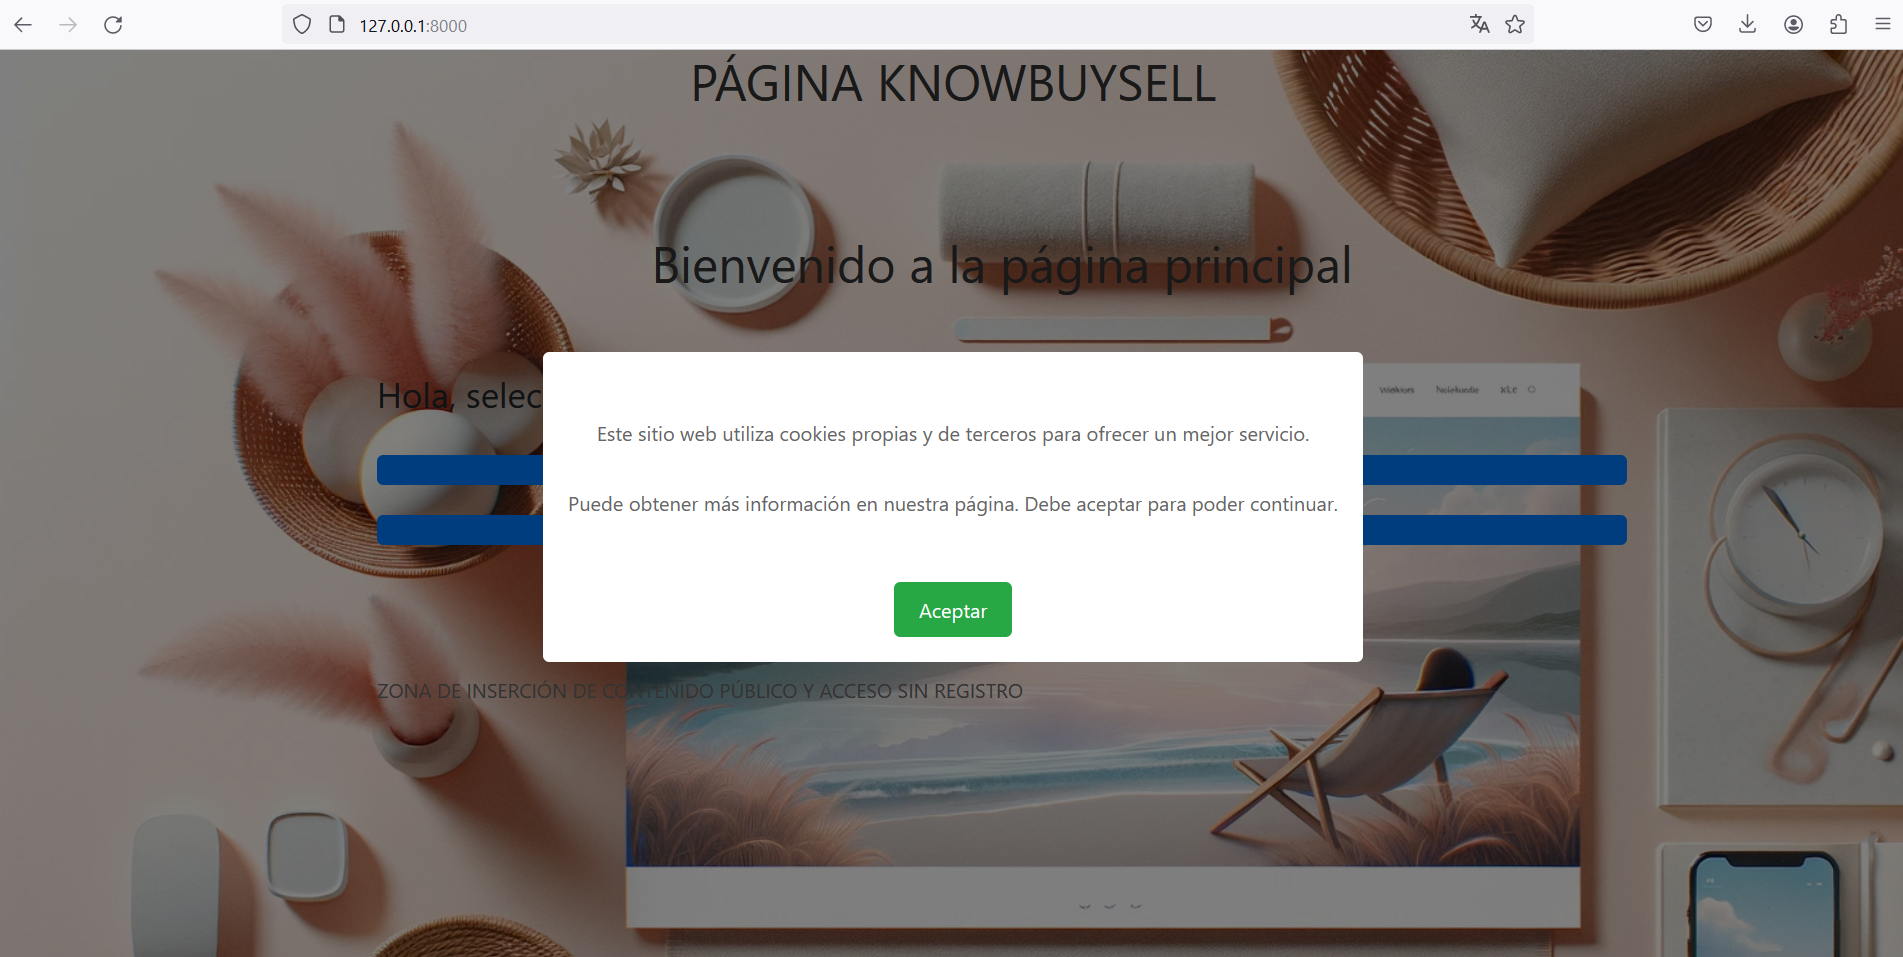
\includegraphics[width=\textwidth]{Figura_1.png}
\caption{\label{fig:1}Página de inicio.}
\end{figure}

Una vez hemos presionsado el botón verde donde se indica aceptar, nos muestra la página de Bienvenida que podemos ver en la Figura \ref{fig:2}.

Tras entrar hemos accedido al apartado ``Inspeccionar'' del botón derecho del del ratón para comprobar que efectivamente se ha guardado el registro de la aceptación de las cookies, esto es importante para cumplir con el reglamento vigente de protección de datos o como son concidas sus siglas en inglés el cumplimient del ``GDPR''. Para ello nos vamos a la Figura \ref{fig:cookie}

\begin{figure}[h]
\centering
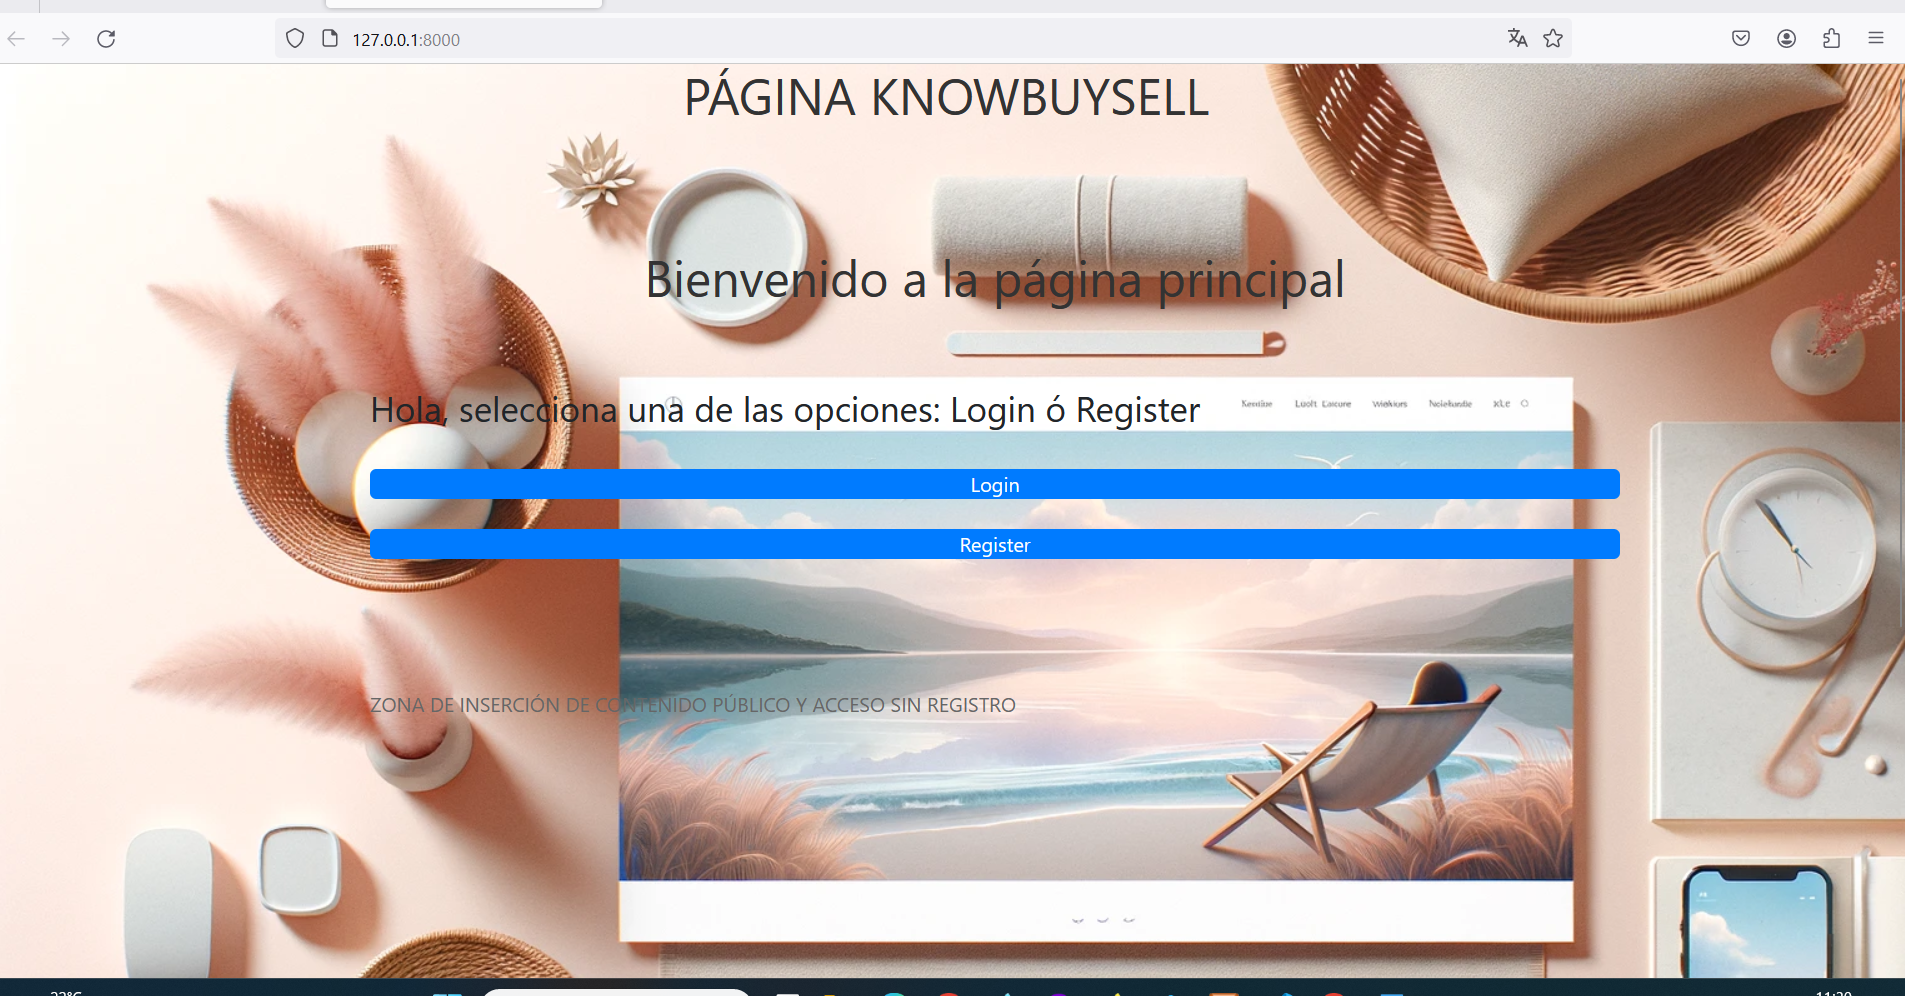
\includegraphics[width=\textwidth]{Figura_2.png}
\caption{\label{fig:2}Página de Bienvenida previa a registro y logo.}
\end{figure}

\begin{figure}[h]
\centering
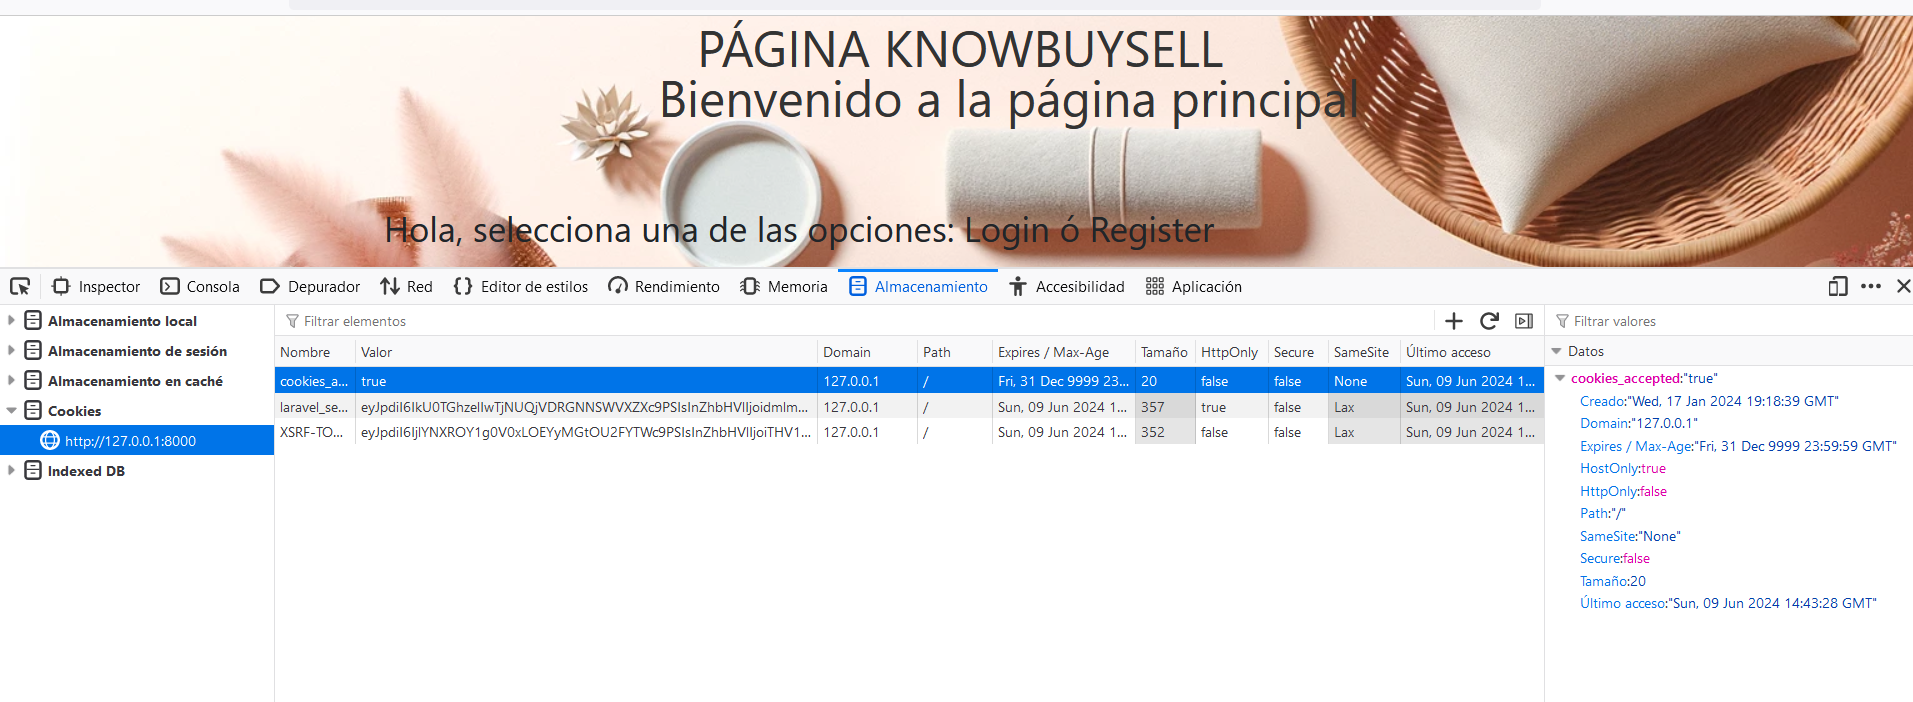
\includegraphics[width=\textwidth]{FiguraCookies.png}
\caption{\label{fig:3}Comprobación de cookies.}
\end{figure}

A continuación la siguiente opción es la de registar una cuenta, en este caso, en el botón ``Register'' permite realizar el registro y en el botón ``Login'' una vez registrado podrá logarse. Ver Figura \ref{fig:2}

Una vez hemos entrado a crear la cuenta de registro, la imagen es la que podemos comprobar en la Figura \ref{fig:4}, donde una vez inluido los datos solicitados presionamos sobre ``Create account''. Y ya tendríamos nuestra cuenta creada, desde esta página podemos acceder al botón ``Login'' para poder logarnos y acceder a la parte privada de la página web, una vez hamos metido nuestro username o dirección de email y nuestro password o clave, como podemos comprobar en la Figura \ref{fig:5}.

\begin{figure}[h]
\centering
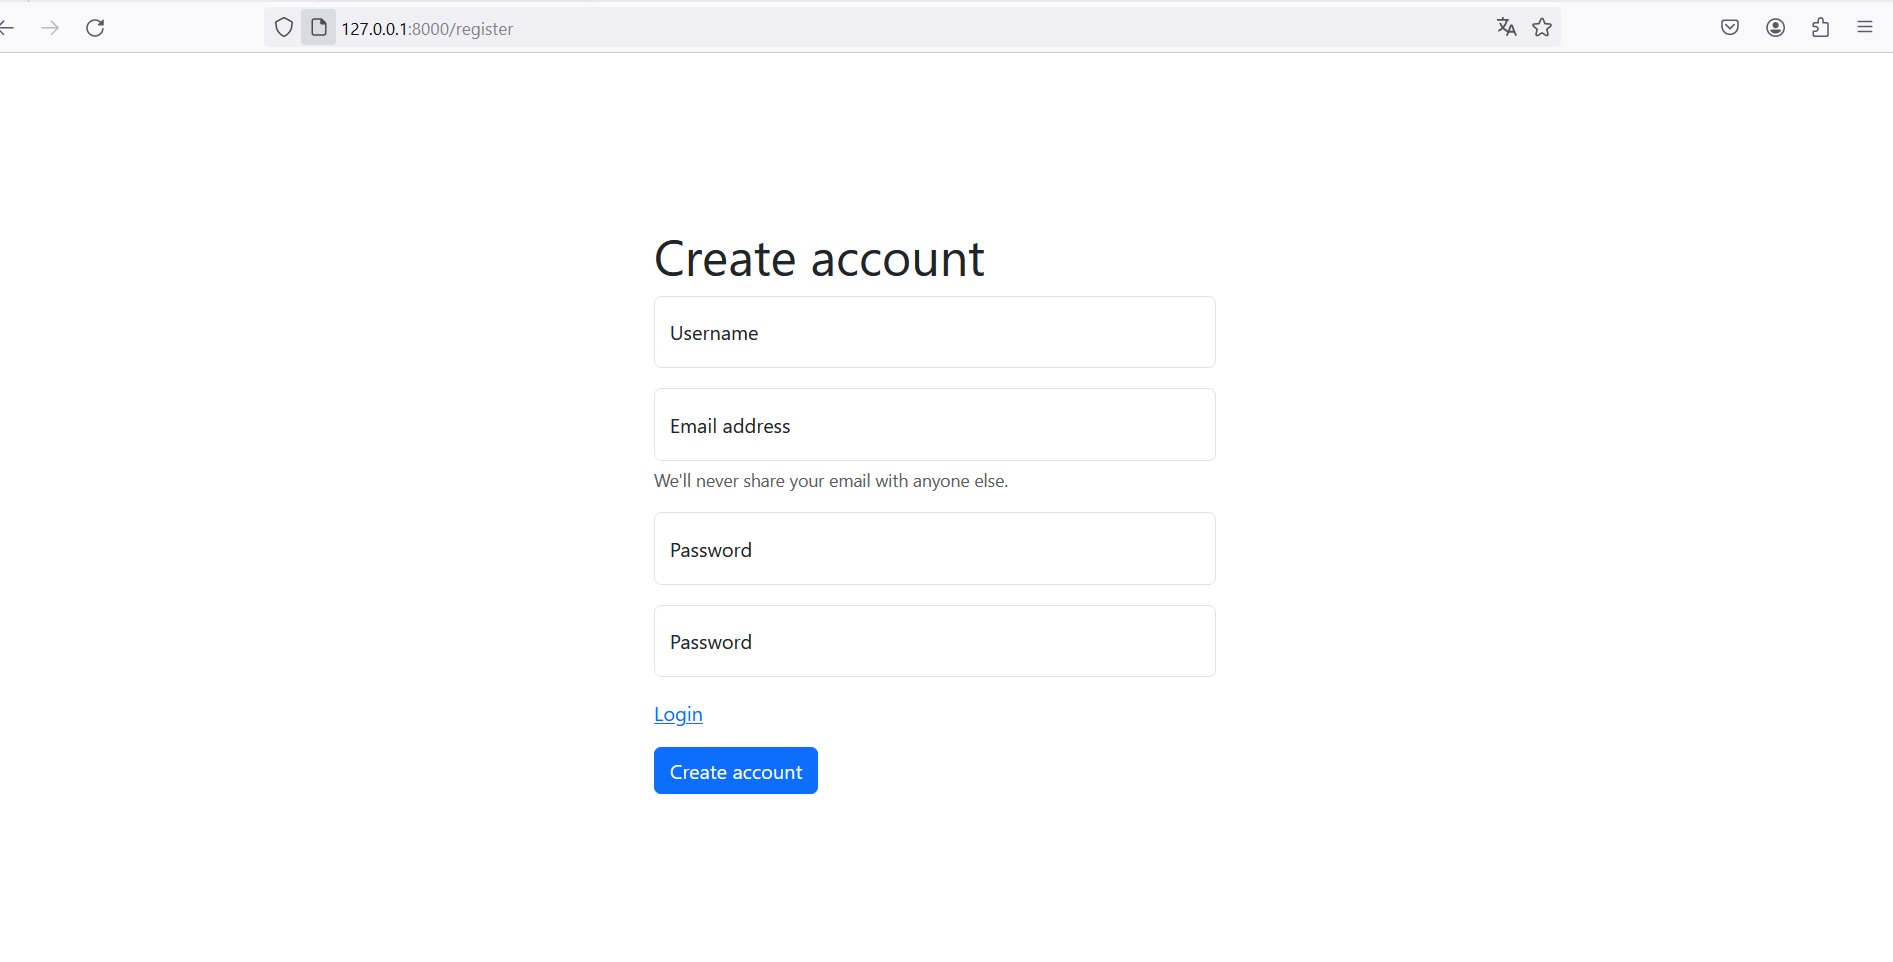
\includegraphics[width=\textwidth]{Figura_3.png}
\caption{\label{fig:4}Página para crear cuenta de usuario.}
\end{figure}

\begin{figure}[h]
\centering
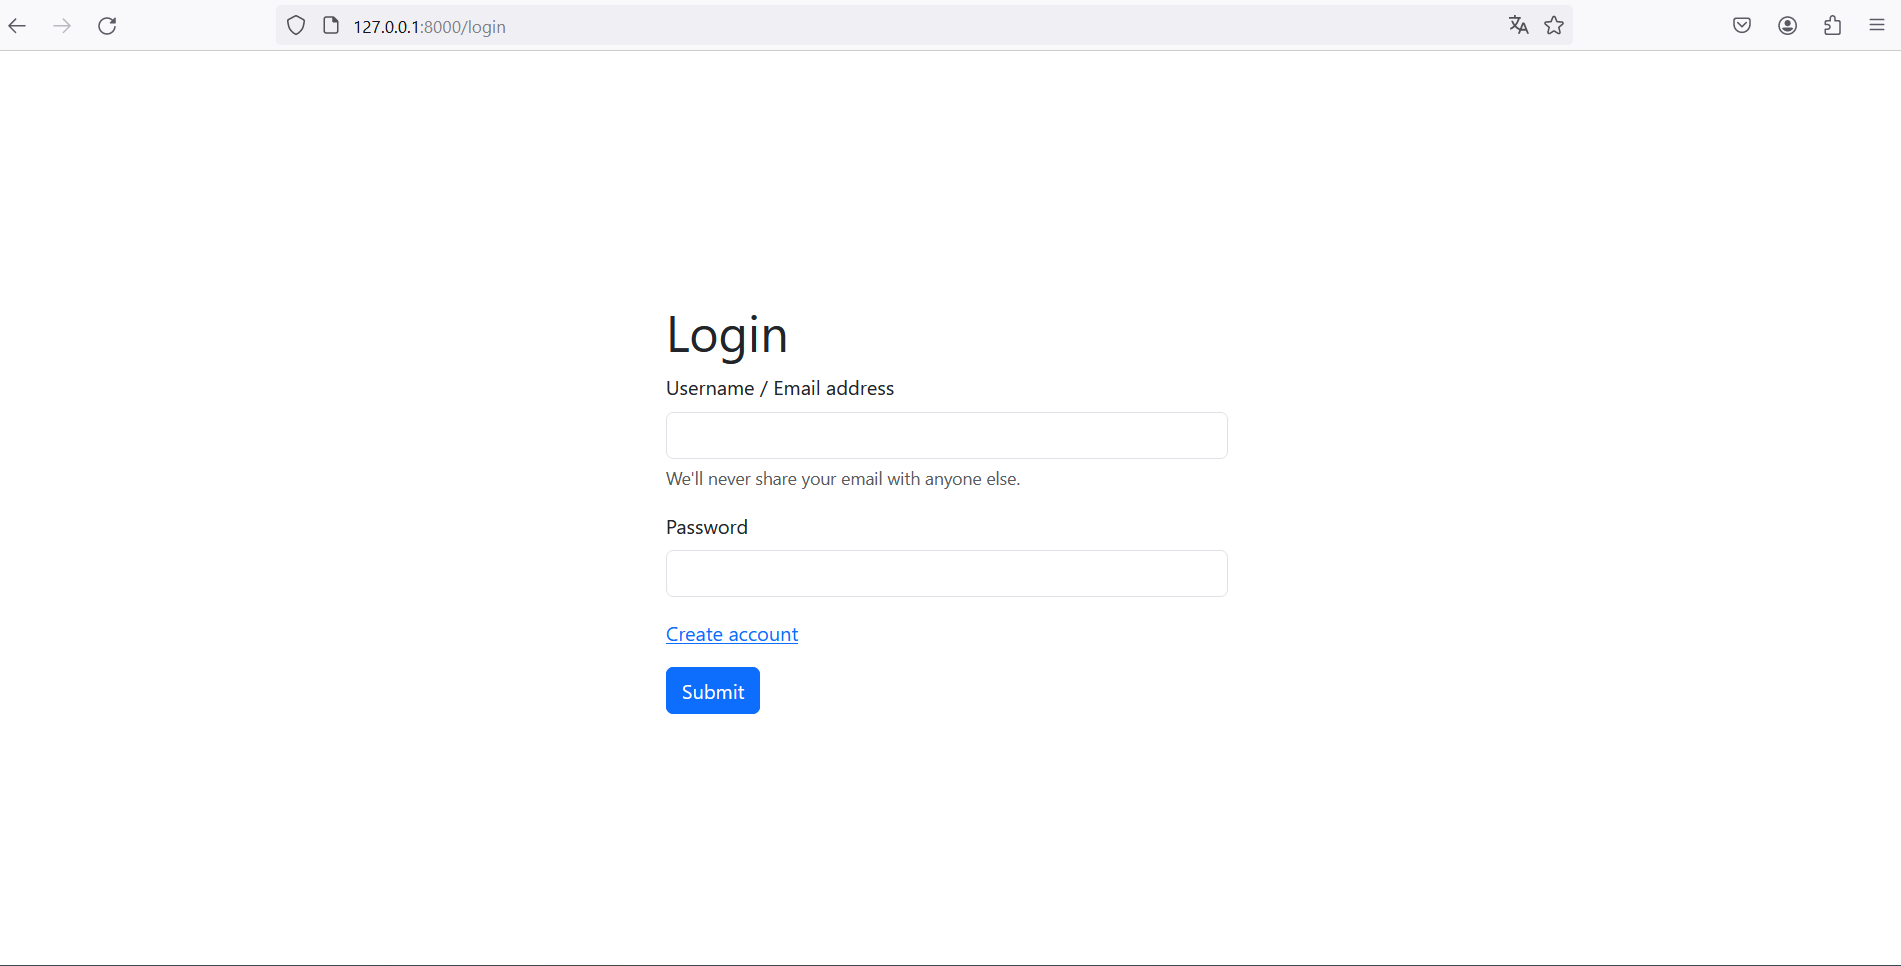
\includegraphics[width=\textwidth]{Figura_4.png}
\caption{\label{fig:5}Página para logarse una vez se creado una cuenta previa.}
\end{figure}

Cuando el usuario ya se ha logado la página web le da la Bienvenida con su nombre, y arriba a la derecha aparece el nombre de usuario y un desplegable donde poder logarse, aunque esto seguirá estando diponible en las siguientes páginas. Ver Figura \ref{fig:6}

Desde este punto si pinchamos en la barra superior encima de la palabra ``Comprar'' la página nos redirige hacia la web donde podemos empezar a realizar compras, ver Figura \ref{fig:7}. En la Figura \ref{fig:8} podemos ver un ejemplo de los productos que se van a comprar. Y una vez seleccionados los productos se aparece el mensaje de ``Compra realizada correctamente'' en la Figura \ref{fig:9}.

\begin{figure}[h]
\centering
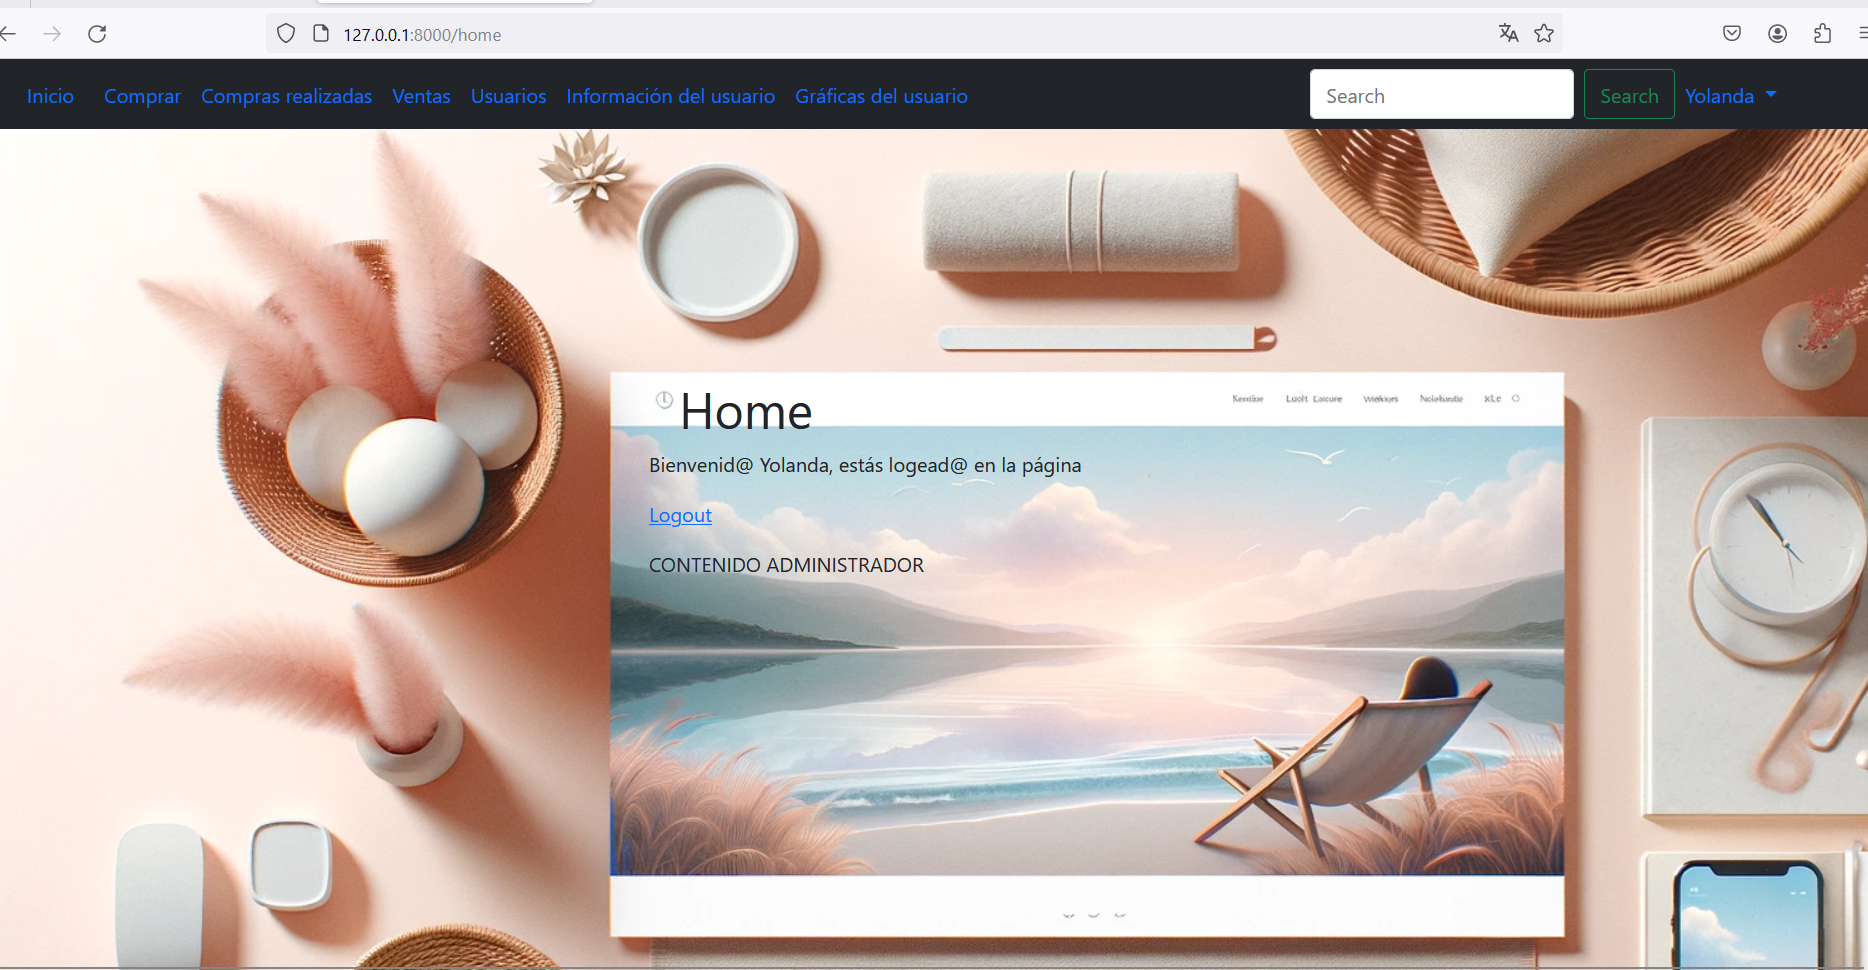
\includegraphics[width=\textwidth]{Figura_5.png}
\caption{\label{fig:6}Página Bienvenida tras logarse.}
\end{figure}

\begin{figure}[h]
\centering
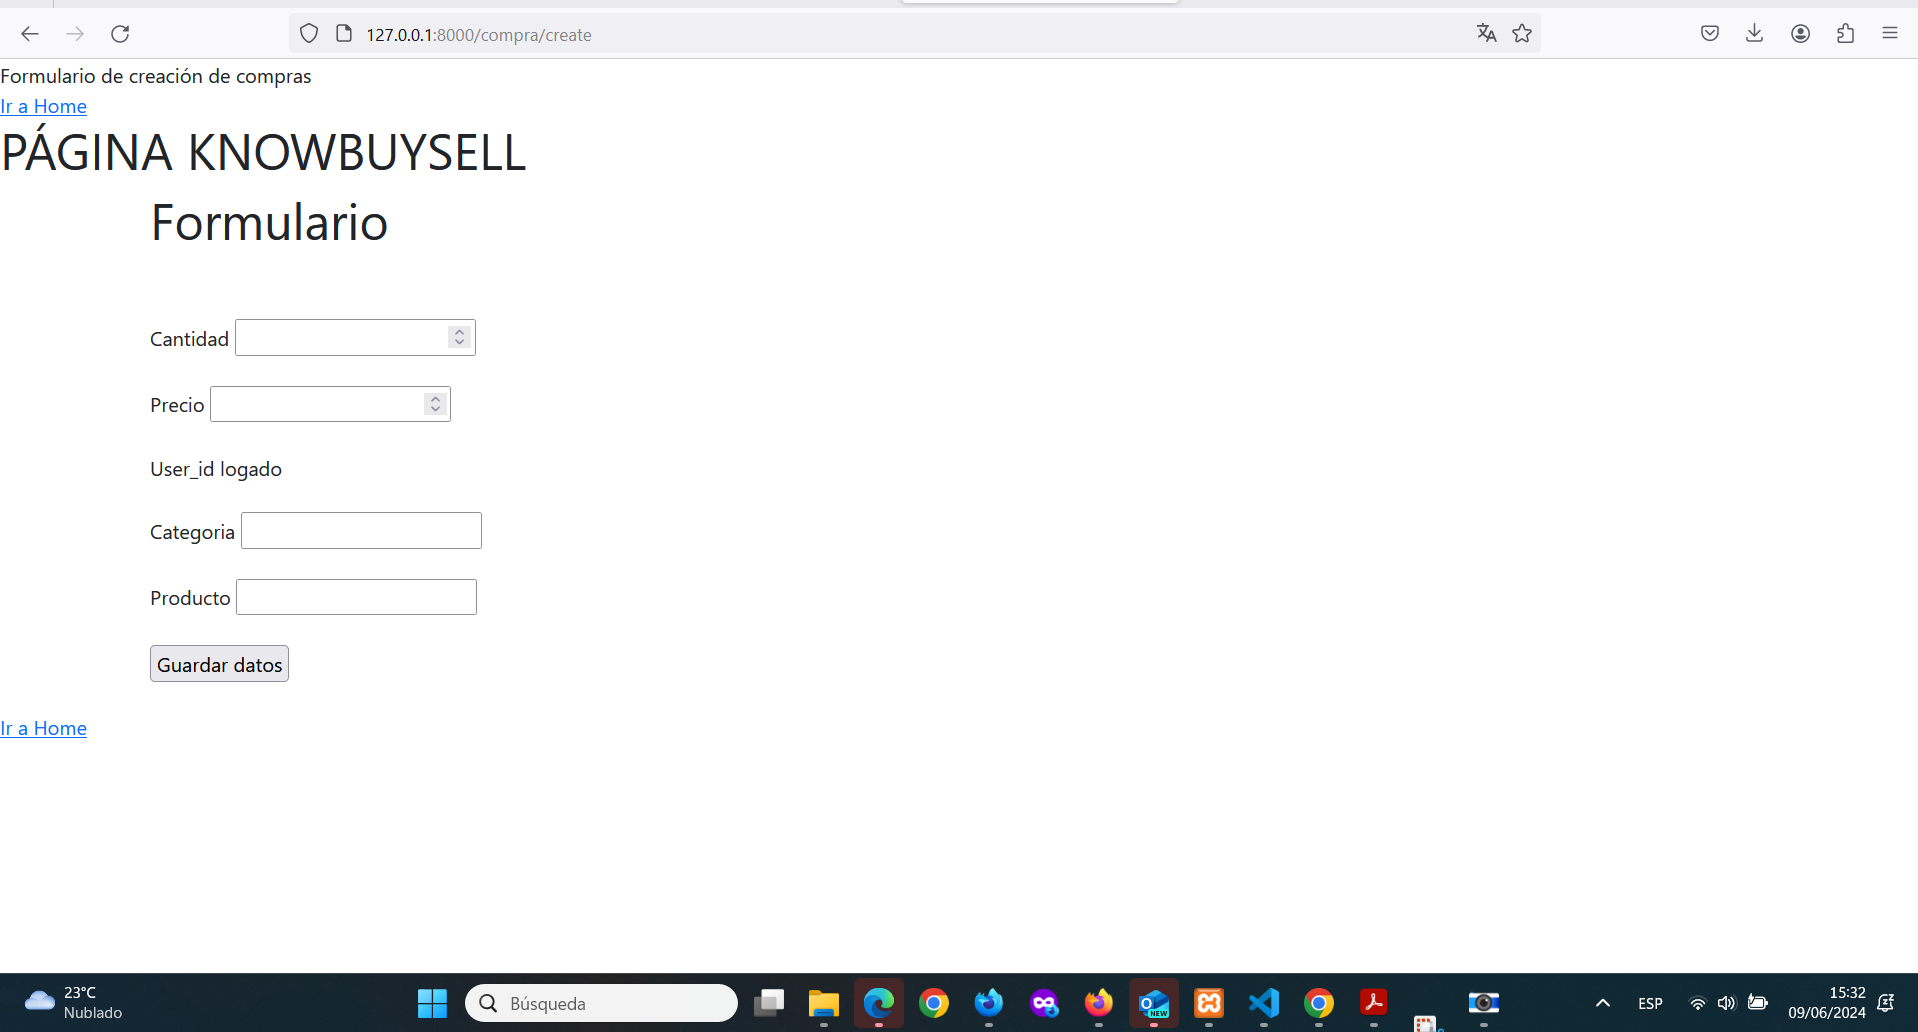
\includegraphics[width=\textwidth]{Figura_6.png}
\caption{\label{fig:7}Página para realizar las compras (CRUD).}
\end{figure}

\begin{figure}[h]
\centering
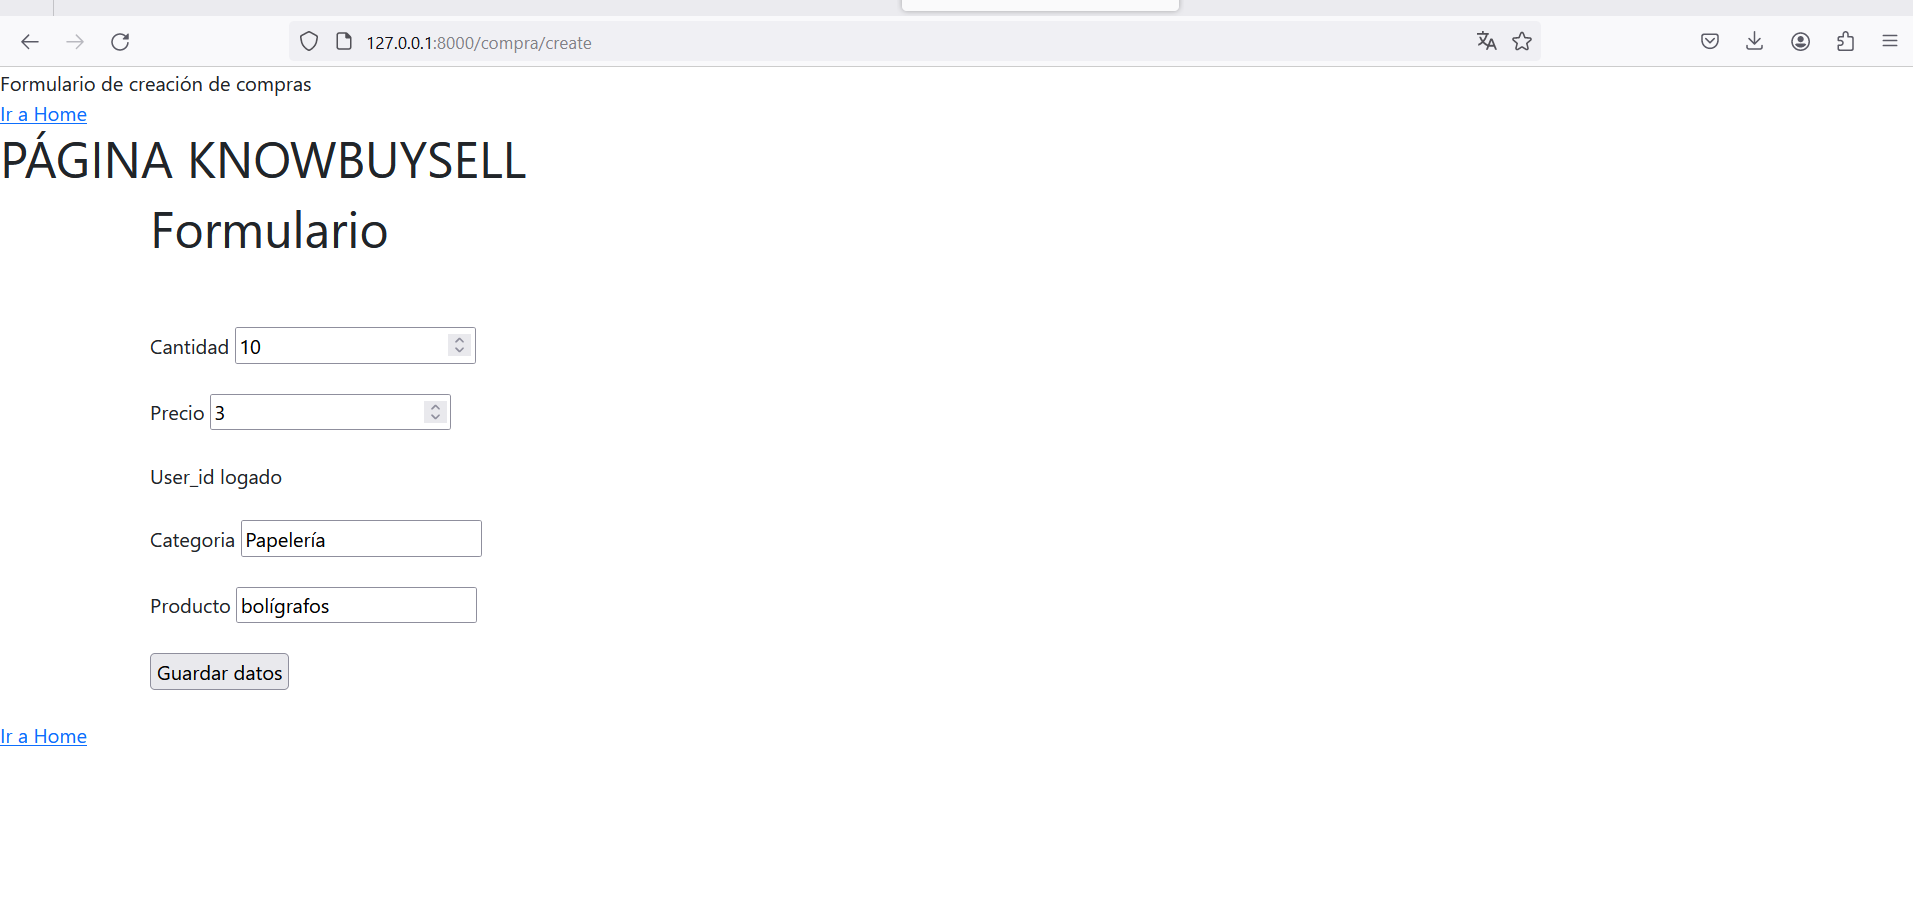
\includegraphics[width=\textwidth]{Figura_7.png}
\caption{\label{fig:8}Página muestra rellenado de datos para la compra (CRUD).}
\end{figure}

En la Figura \ref{fig:10} se muestran todos los productos desde la vista del administrador, en caso de que el usuario no fuera administrador, sólo se mostraría los datos del usuario logado en concreto.
En cuanto a la Figura \ref{fig:11} creamos esta página para mostrar todas las compras pero por grupos de ventas es decirm por cada compra los productos comprados y realizado en una fecha determinada y por grupo de compra. (Por el momento no está habilitada esta información)
\begin{figure}[h]
\centering
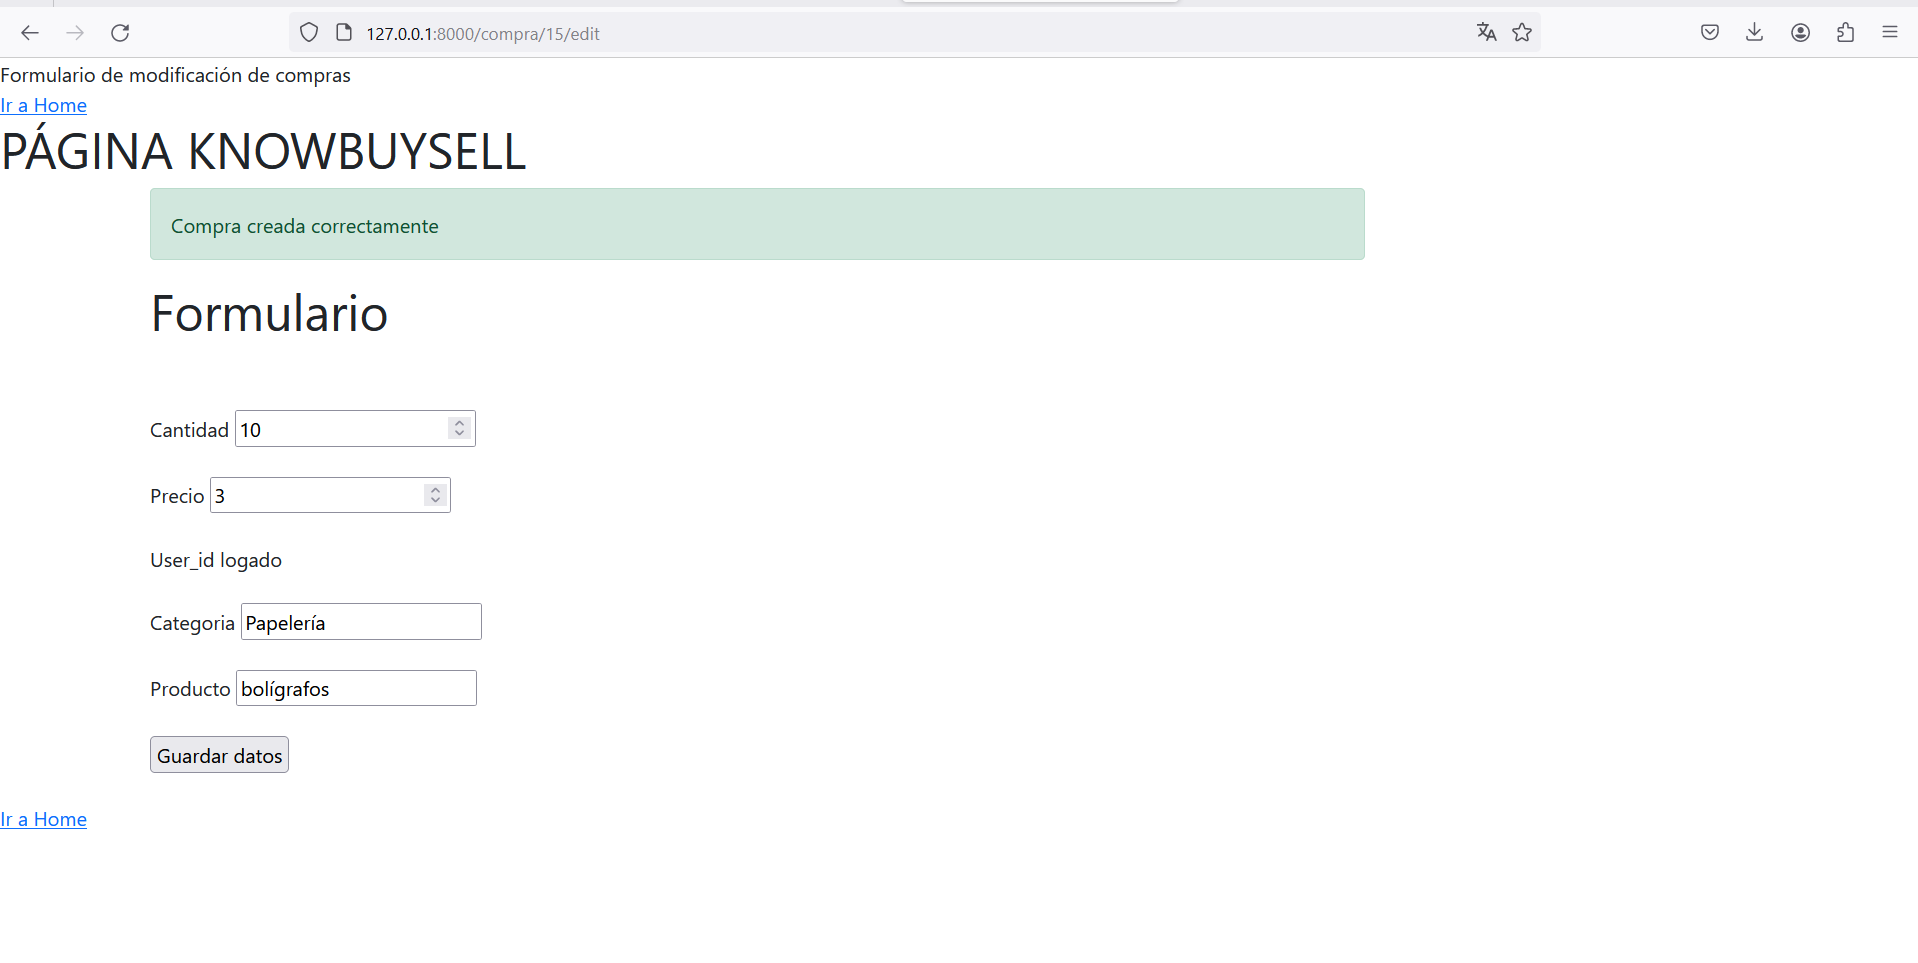
\includegraphics[width=\textwidth]{Figura_8.png}
\caption{\label{fig:9}Página donde se muestra que la compra se realizado correctamente.}
\end{figure}

\begin{figure}[h]
\centering
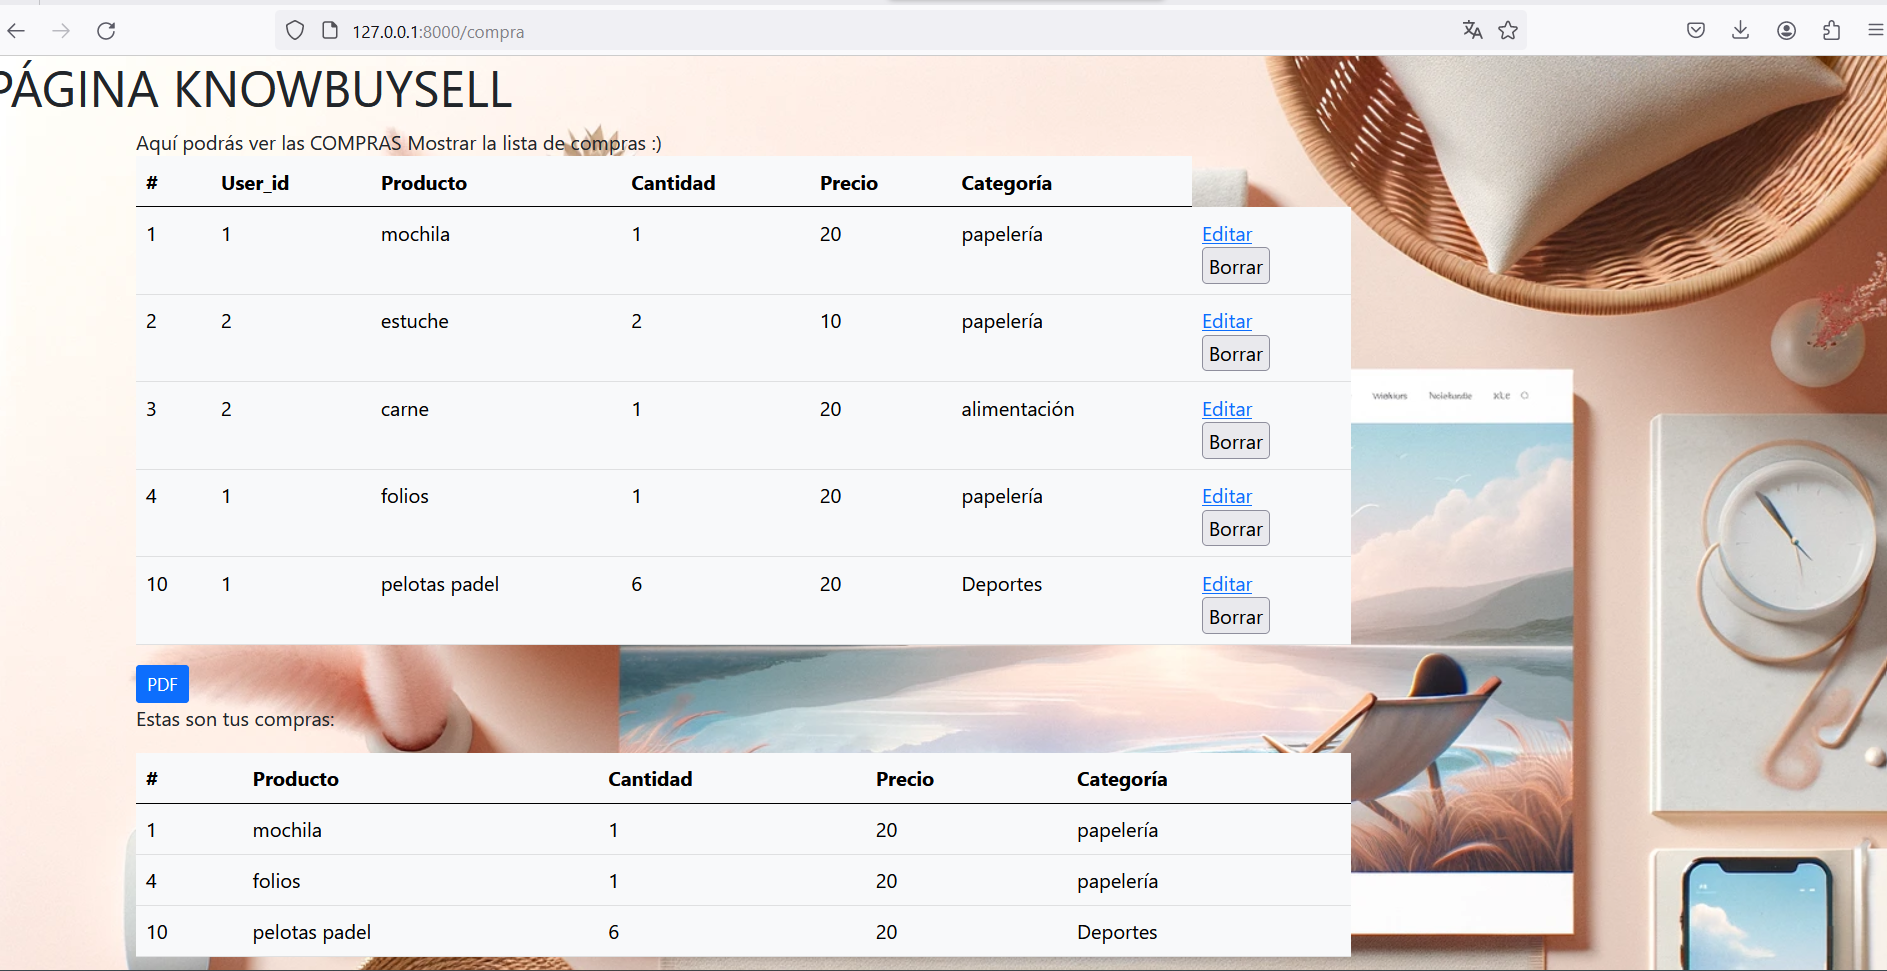
\includegraphics[width=\textwidth]{Figura_9.png}
\caption{\label{fig:10}Reporte de información de compras y de creación de documento PDF. Información, modificación y eliminación de compras (CRUD).}
\end{figure}

A través del acceso de administrador en el apartado ``usuarios'' podemos acceder al listado de usuarios registrados en la página web. Si quien accede no es adminsitrador, simplemente no vería ninguna información, ver Figura \ref{fig:12}. Es en la página que muestra la Figura \ref{fig:13} donde el usuario tiene acceso a sus datos de email. Y si queremos meter más información del usuario sería en esta parte de la aplicación web.

Finalmente en el apartado ``Gráficas del usuario'' es donde tanto el usuario como el administrador pueden acceder a la información por porcentajes a través de las gráficas para obtener la información, finalidad de proyecto en cuestión. (Nota: actualmente se está realizando la mejora para que se muestren los datos de forma más correcta)


\begin{figure}[h]
\centering
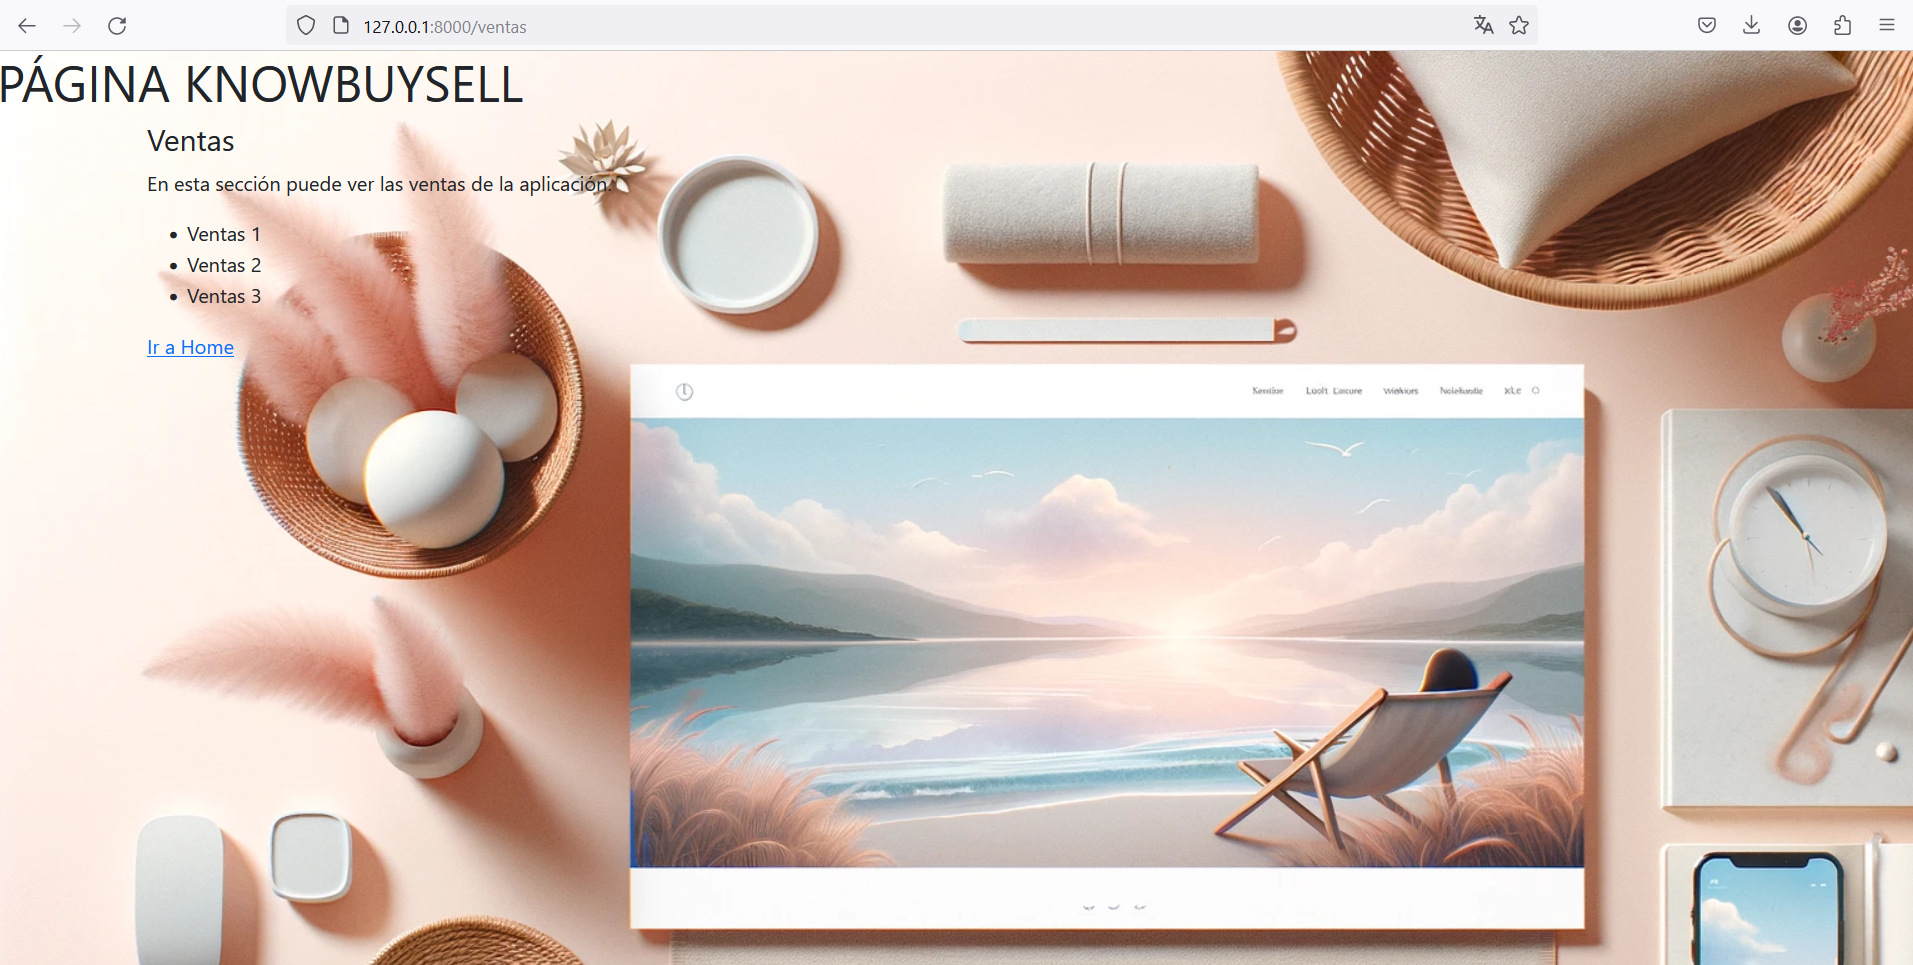
\includegraphics[width=\textwidth]{Figura_10.png}
\caption{\label{fig:11}Página ventas.}
\end{figure}

\begin{figure}[h]
\centering
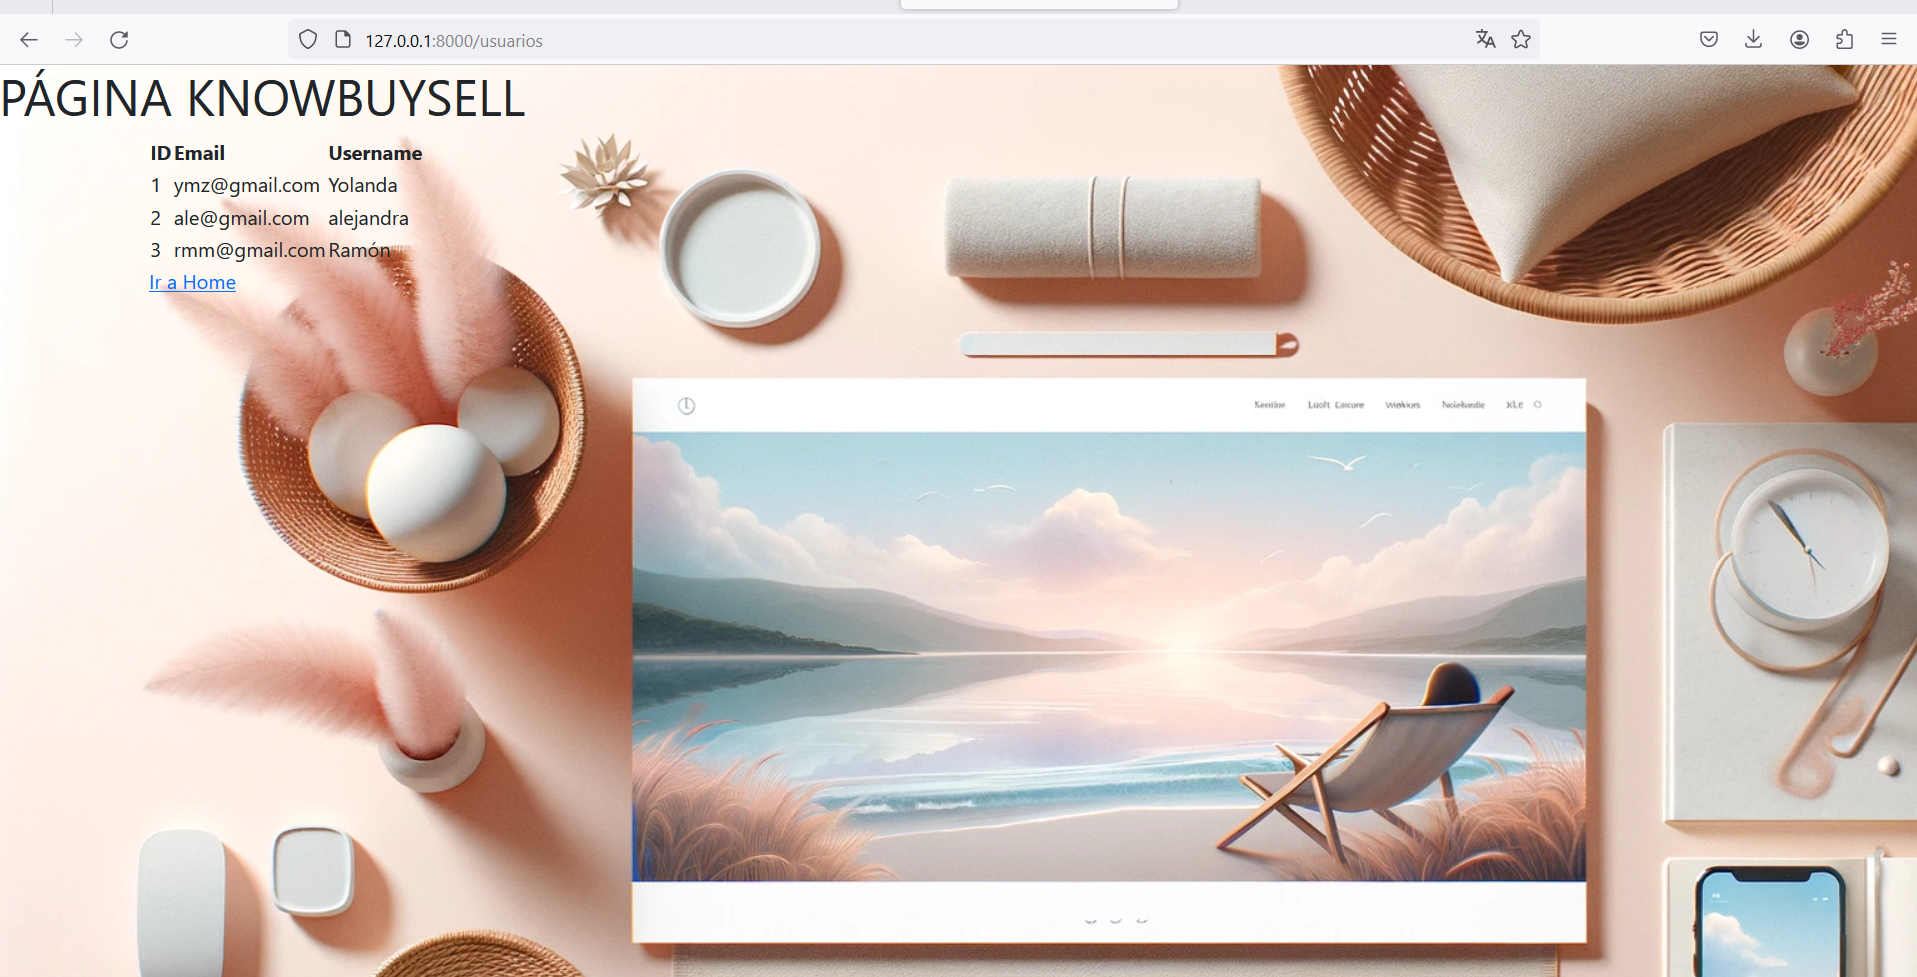
\includegraphics[width=\textwidth]{Figura_11.png}
\caption{\label{fig:12}Página información usuarios (sólo tiene acceso el administrador).}
\end{figure}

\begin{figure}[h]
\centering
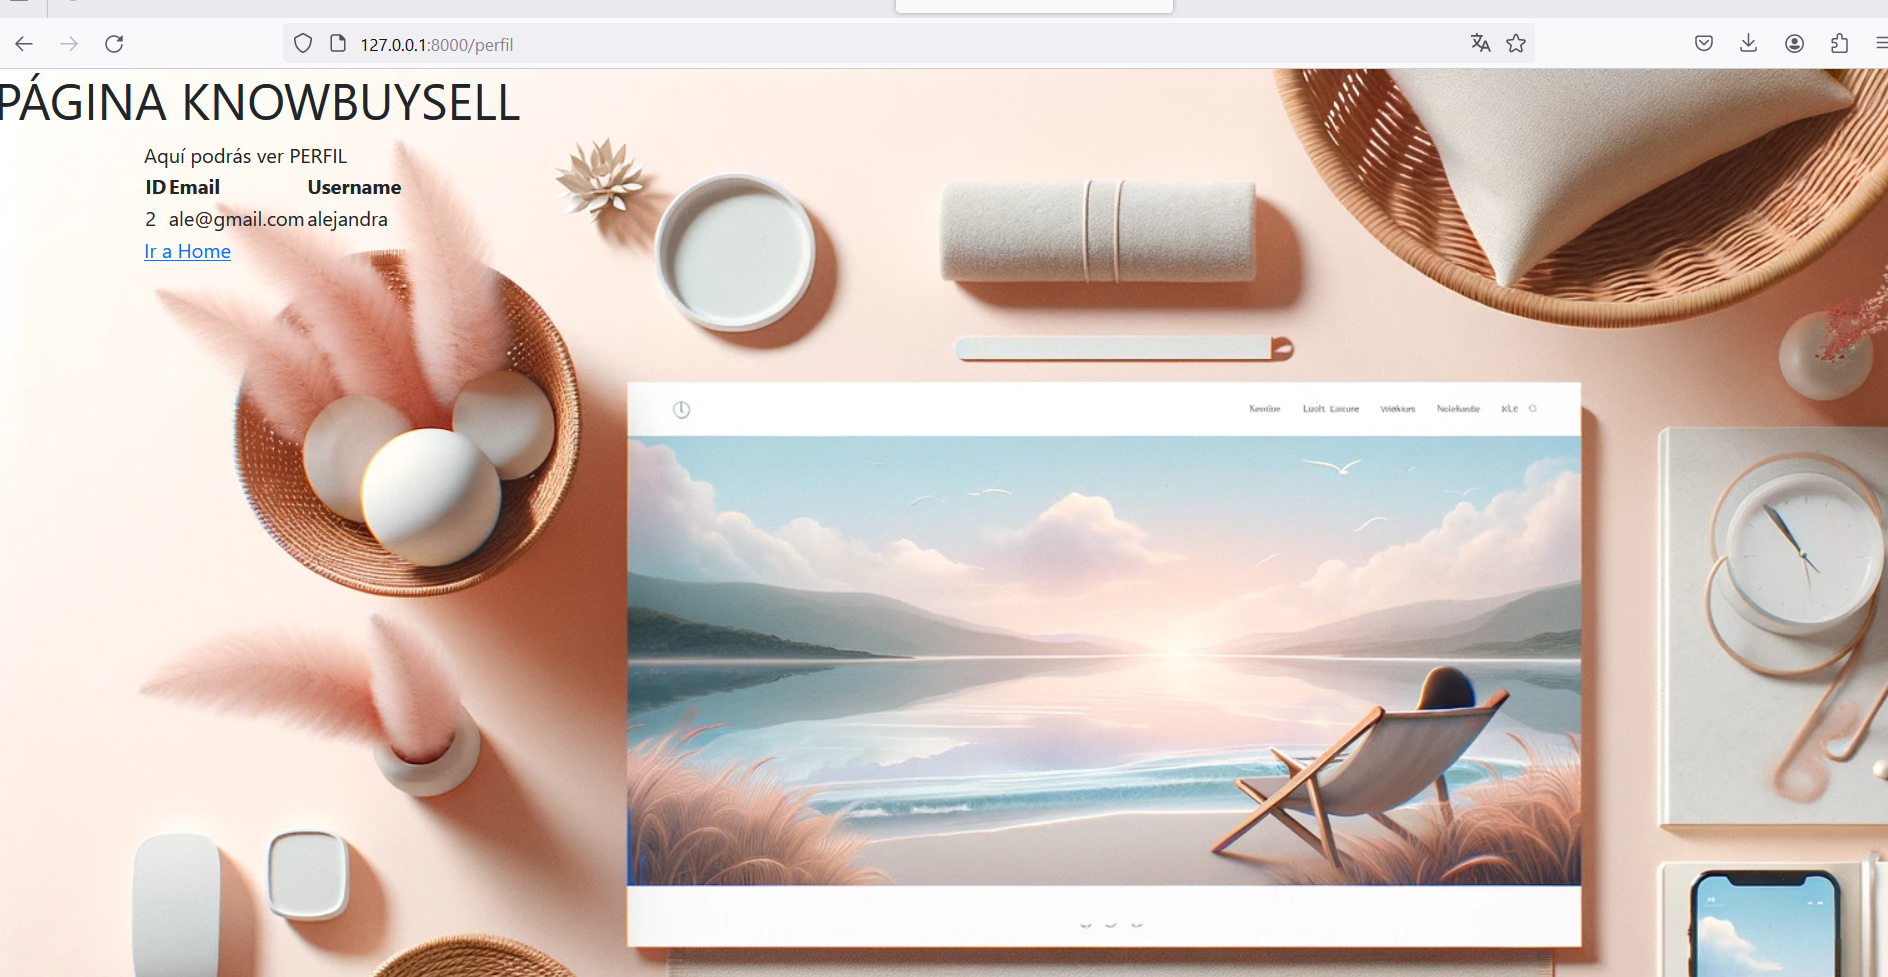
\includegraphics[width=\textwidth]{Figura_12.png}
\caption{\label{fig:13}Página perfil (Cada usuario accede a la información de sus datos).}
\end{figure}

\begin{figure}[h]
\centering
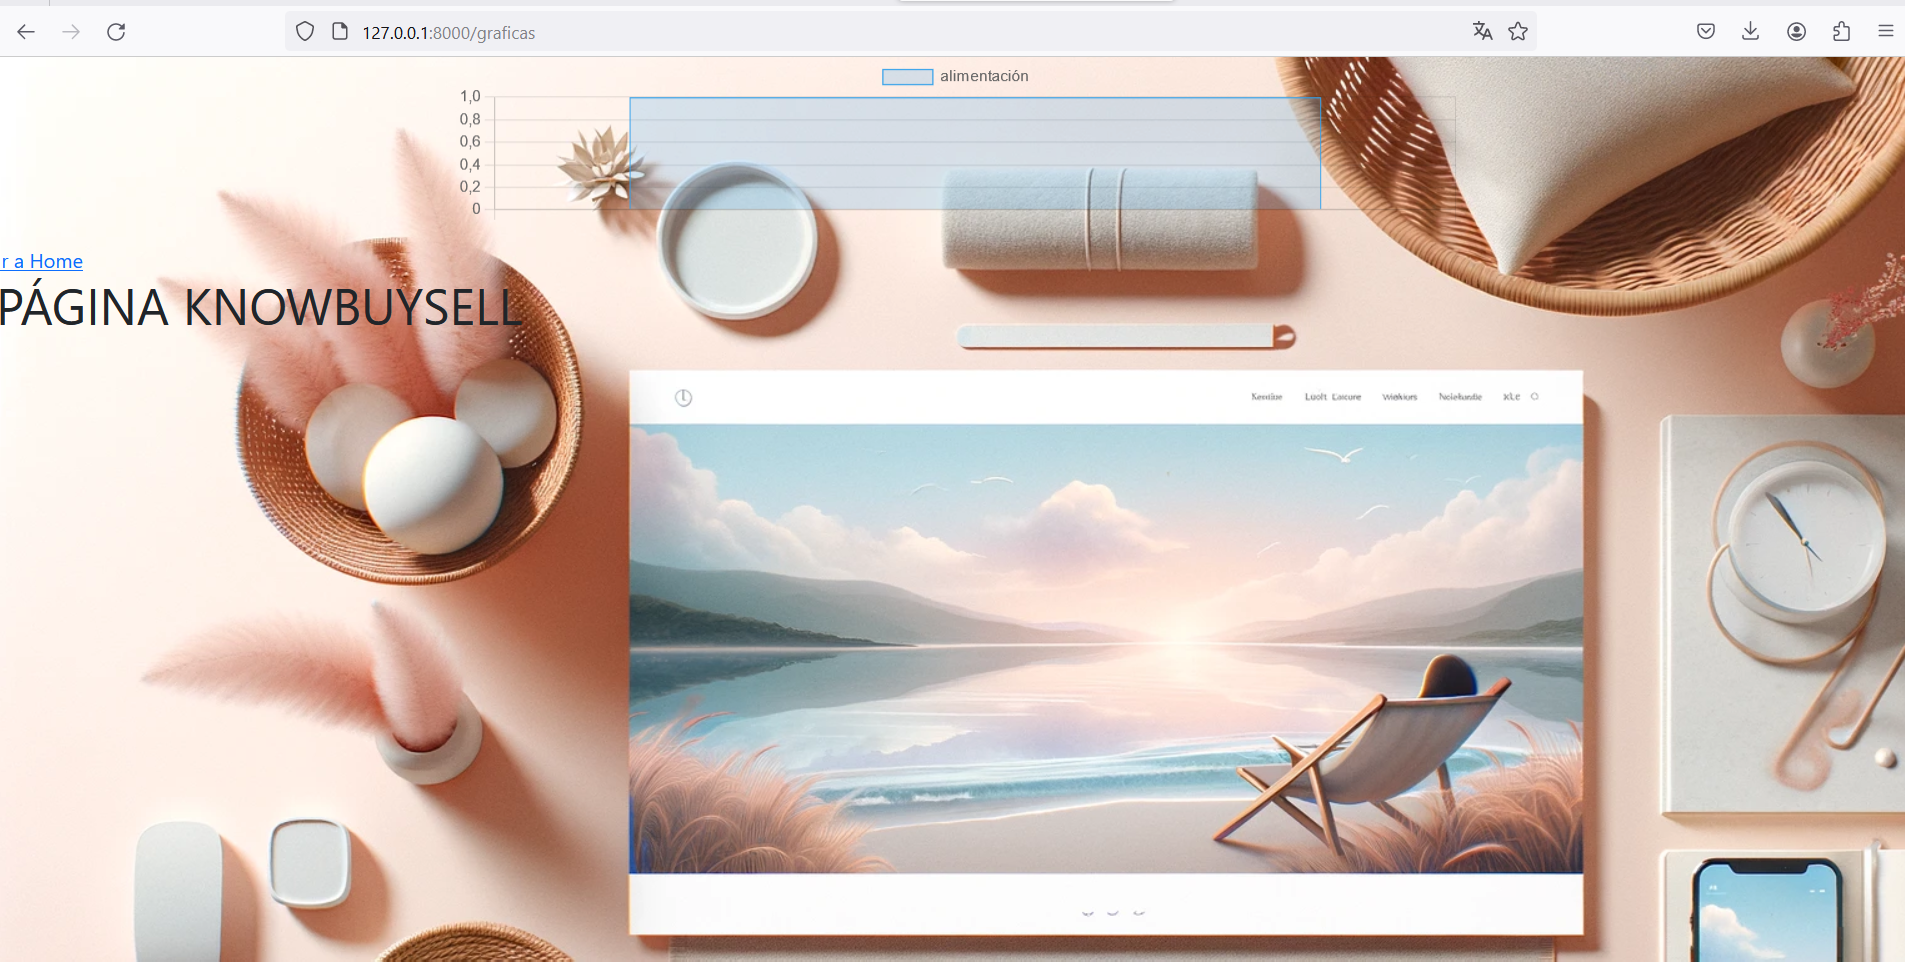
\includegraphics[width=\textwidth]{Figura_13.png}
\caption{\label{fig:14}Página gráfica.}
\end{figure}

% \bibliographystyle{alpha}
% \bibliography{sample}
\end{document}